\section{Contraposée du théorème de Thalès}
    \subsection{Énoncé}
        \begin{theoreme}[\admis]
            Si dans une configuration géométrique :
            \begin{itemize}
                \item Deux droites $(d)$ et $(d')$ sont sécantes en un point $A$.
                \item $B$ et $M$ sont deux points de la droites $(d)$, distincts de A.
                \item $C$ et $N$ sont deux points de la droite $(d')$, distincts de $A$.
                \item $\dfrac{AM}{AB} \neq \dfrac{AN}{AC}$.       
            \end{itemize}
            \medskip
            alors les droites $(BC)$ et $(MN)$ ne sont pas parallèles.
        \end{theoreme}

    \subsection{Exemple de rédaction}

        \begin{methode*1}[Justifier que deux droites ne sont pas parallèles]
            \begin{multicols}2
                \begin{itemize}
                    \item Déterminer les droites sécantes.                    
                    \item Identifier les deux triangles.
                    \columnbreak                    
                    \item Calculer les rapports de longueurs non portées par les droites candidates.
                    \item Invoquer la contraposée du théorème de Thalès ou le théorème lui-même.
                \end{itemize}
            \end{multicols}

            \exercice

            \begin{minipage}{8cm}
                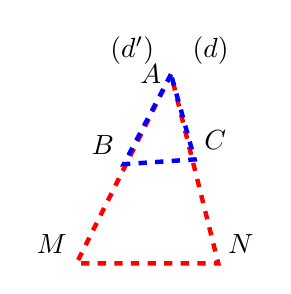
\begin{tikzpicture}[scale = 0.3]
                    % \draw[help lines, color=black!30, dashed] (0,0) grid (12,14);        
                    \coordinate[label=left:$A$] (A) at (7,13);
                    \coordinate[label=left:$(d')$] (d') at (6.7,14);
                    \coordinate[label=right:$(d)$] (d) at (7.5,14);
                    \coordinate[label=above right:$N$] (N) at (9,5);
                    \coordinate[label=above left:$M$] (M) at (3,5);
                    \coordinate[label=above left:$B$] (B) at (5,9.2);
                    \coordinate (M1) at (4,5);
                    \coordinate[label=above right:$C$] (C) at (8,9.4);
                    \coordinate (N1) at (10,5);
        
                    \tkzDrawLine(A,M);
                    \tkzDrawLine(A,N);
                    \tkzDrawLine(M,N);
                    \tkzDrawLine(B,C);
                    \tkzDrawLine(M1,N1);     
                    \draw[dashed, color=red, ultra thick] (A)--(M)--(N)--(A);
                    \draw[dashed, color=blue, ultra thick] (A)--(B)--(C)--(A);
                \end{tikzpicture}
            \end{minipage}
            \begin{minipage}{8cm}
                \begin{itemize}
                    \item Les droites $(d)$ et $(d')$ se coupent en $A$.
                    \item $AB=\Lg{11.9}$ ; $AM=\Lg{35}$. 
                    \item $AC=\Lg{18.2}$ ; $AN=\Lg{52}$.
                \end{itemize}

                % \vspace*{1cm}
                Démontrer que les droites $(MN)$ et $(BC)$ 
                
                ne sont pas parallèles.
            \end{minipage}
            
            \correction
            Dans la configuration ci-dessus : 
            \begin{itemize}
                \item les droites $(MB)$ et $(CN)$ sont sécantes en $A$.                
                \item les deux triangles sont \textcolor{red}{$AMN$} et \textcolor{blue}{$ABC$}.            
                \item D'une part $\dfrac{\textcolor{blue}{AB}}{\textcolor{red}{AM}} = \dfrac{\textcolor{blue}{11,9}}{\textcolor{red}{35}}=0,34$
                \hfill
                D'autre part $\dfrac{\textcolor{blue}{AC}}{\textcolor{red}{AN}} = \dfrac{\textcolor{blue}{18,2}}{\textcolor{red}{52}}=0,35$
            \end{itemize}

            \begin{remarque}
                Les deux rédactions suivantes sont valables.
            \end{remarque}
            
            \hspace*{0.5cm}

            \begin{minipage}{8cm}
                \textbf{or}, si le droites $(MN)$ et $(BC)$ étaient parallèles, d'après le théorème de Thalès, il y aurait égalité des deux rapports
                précédents. Comme ce n'est pas le cas, c'est que \psshadowbox{les droites $(MN)$ et $(BC)$ ne sont pas parallèles}.
    
            \end{minipage}
            \hspace*{0.5cm}
            \vrule
            \hspace*{0.5cm}
            \begin{minipage}{8cm}
                Les rapports précédents étant différents, d'après la contraposée du théorème de Thalès, on peut conclure que \psshadowbox{les droites $(MN)$ et $(BC)$ ne sont pas parallèles}.
            \end{minipage}
        \end{methode*1}

